\documentclass[11pt]{article}
%\usepackage[ansinew]{inputenc} % Acepta caracteres en castellano
%\usepackage[spanish]{babel}    % silabea palabras castellanas
\usepackage{amsmath}
\usepackage{amsfonts}
\usepackage{amssymb}
\usepackage[colorlinks=true,urlcolor=blue,linkcolor=blue,citecolor=blue]{hyperref} % navega por el doc
\usepackage{graphicx}
\usepackage{geometry}           % See geometry.pdf to learn the layout options.
\geometry{letterpaper}
\usepackage{subfigure}           % ... or a4paper or a5paper or ... 
%\geometry{landscape}           % Activate for for rotated page geometry
%\usepackage[parfill]{parskip}  % Activate to begin paragraphs with an empty line rather than an indent
\usepackage{epstopdf}\DeclareGraphicsRule{.tif}{png}{.png}{`convert #1 `dirname #1`/`basename #1 .tif`.png}

\title{LAGO Colombia}
\author{LAGO Collaboration 3.0}
%\date{}                                           % Activate to display a given date or no date

\begin{document}
\maketitle
\section{Detector Description}

\subsection{Instrumentation Description}
Colombia WCD, Guane-3, share similar characteristics with other LAGO WCDs. Located at 
Bucaramanga-Santander (7.140143 lat, -73.121904 long and 956masl), it is a 
cylindrical reservoir filled with high quality purified water up to a level 
of 55 cm, and 103 cm of radio, and with a area of detection of 2.61m$^2$. 
The water is contained in a reflective and diffusive bag, made of Tyvek$^@$.
The water volume is overlooked by a single Hamamatsu photomultiplier tube of $8''$ 
(Ref: R5912) with a 25 \% efficiency at 400nm (see Fig \ref{Guane3WCD}). This is the third generation WCD built and calibrated at Universidad Industrial de Santander\cite{Suarez2011}. 
\begin{figure}
\begin{center}
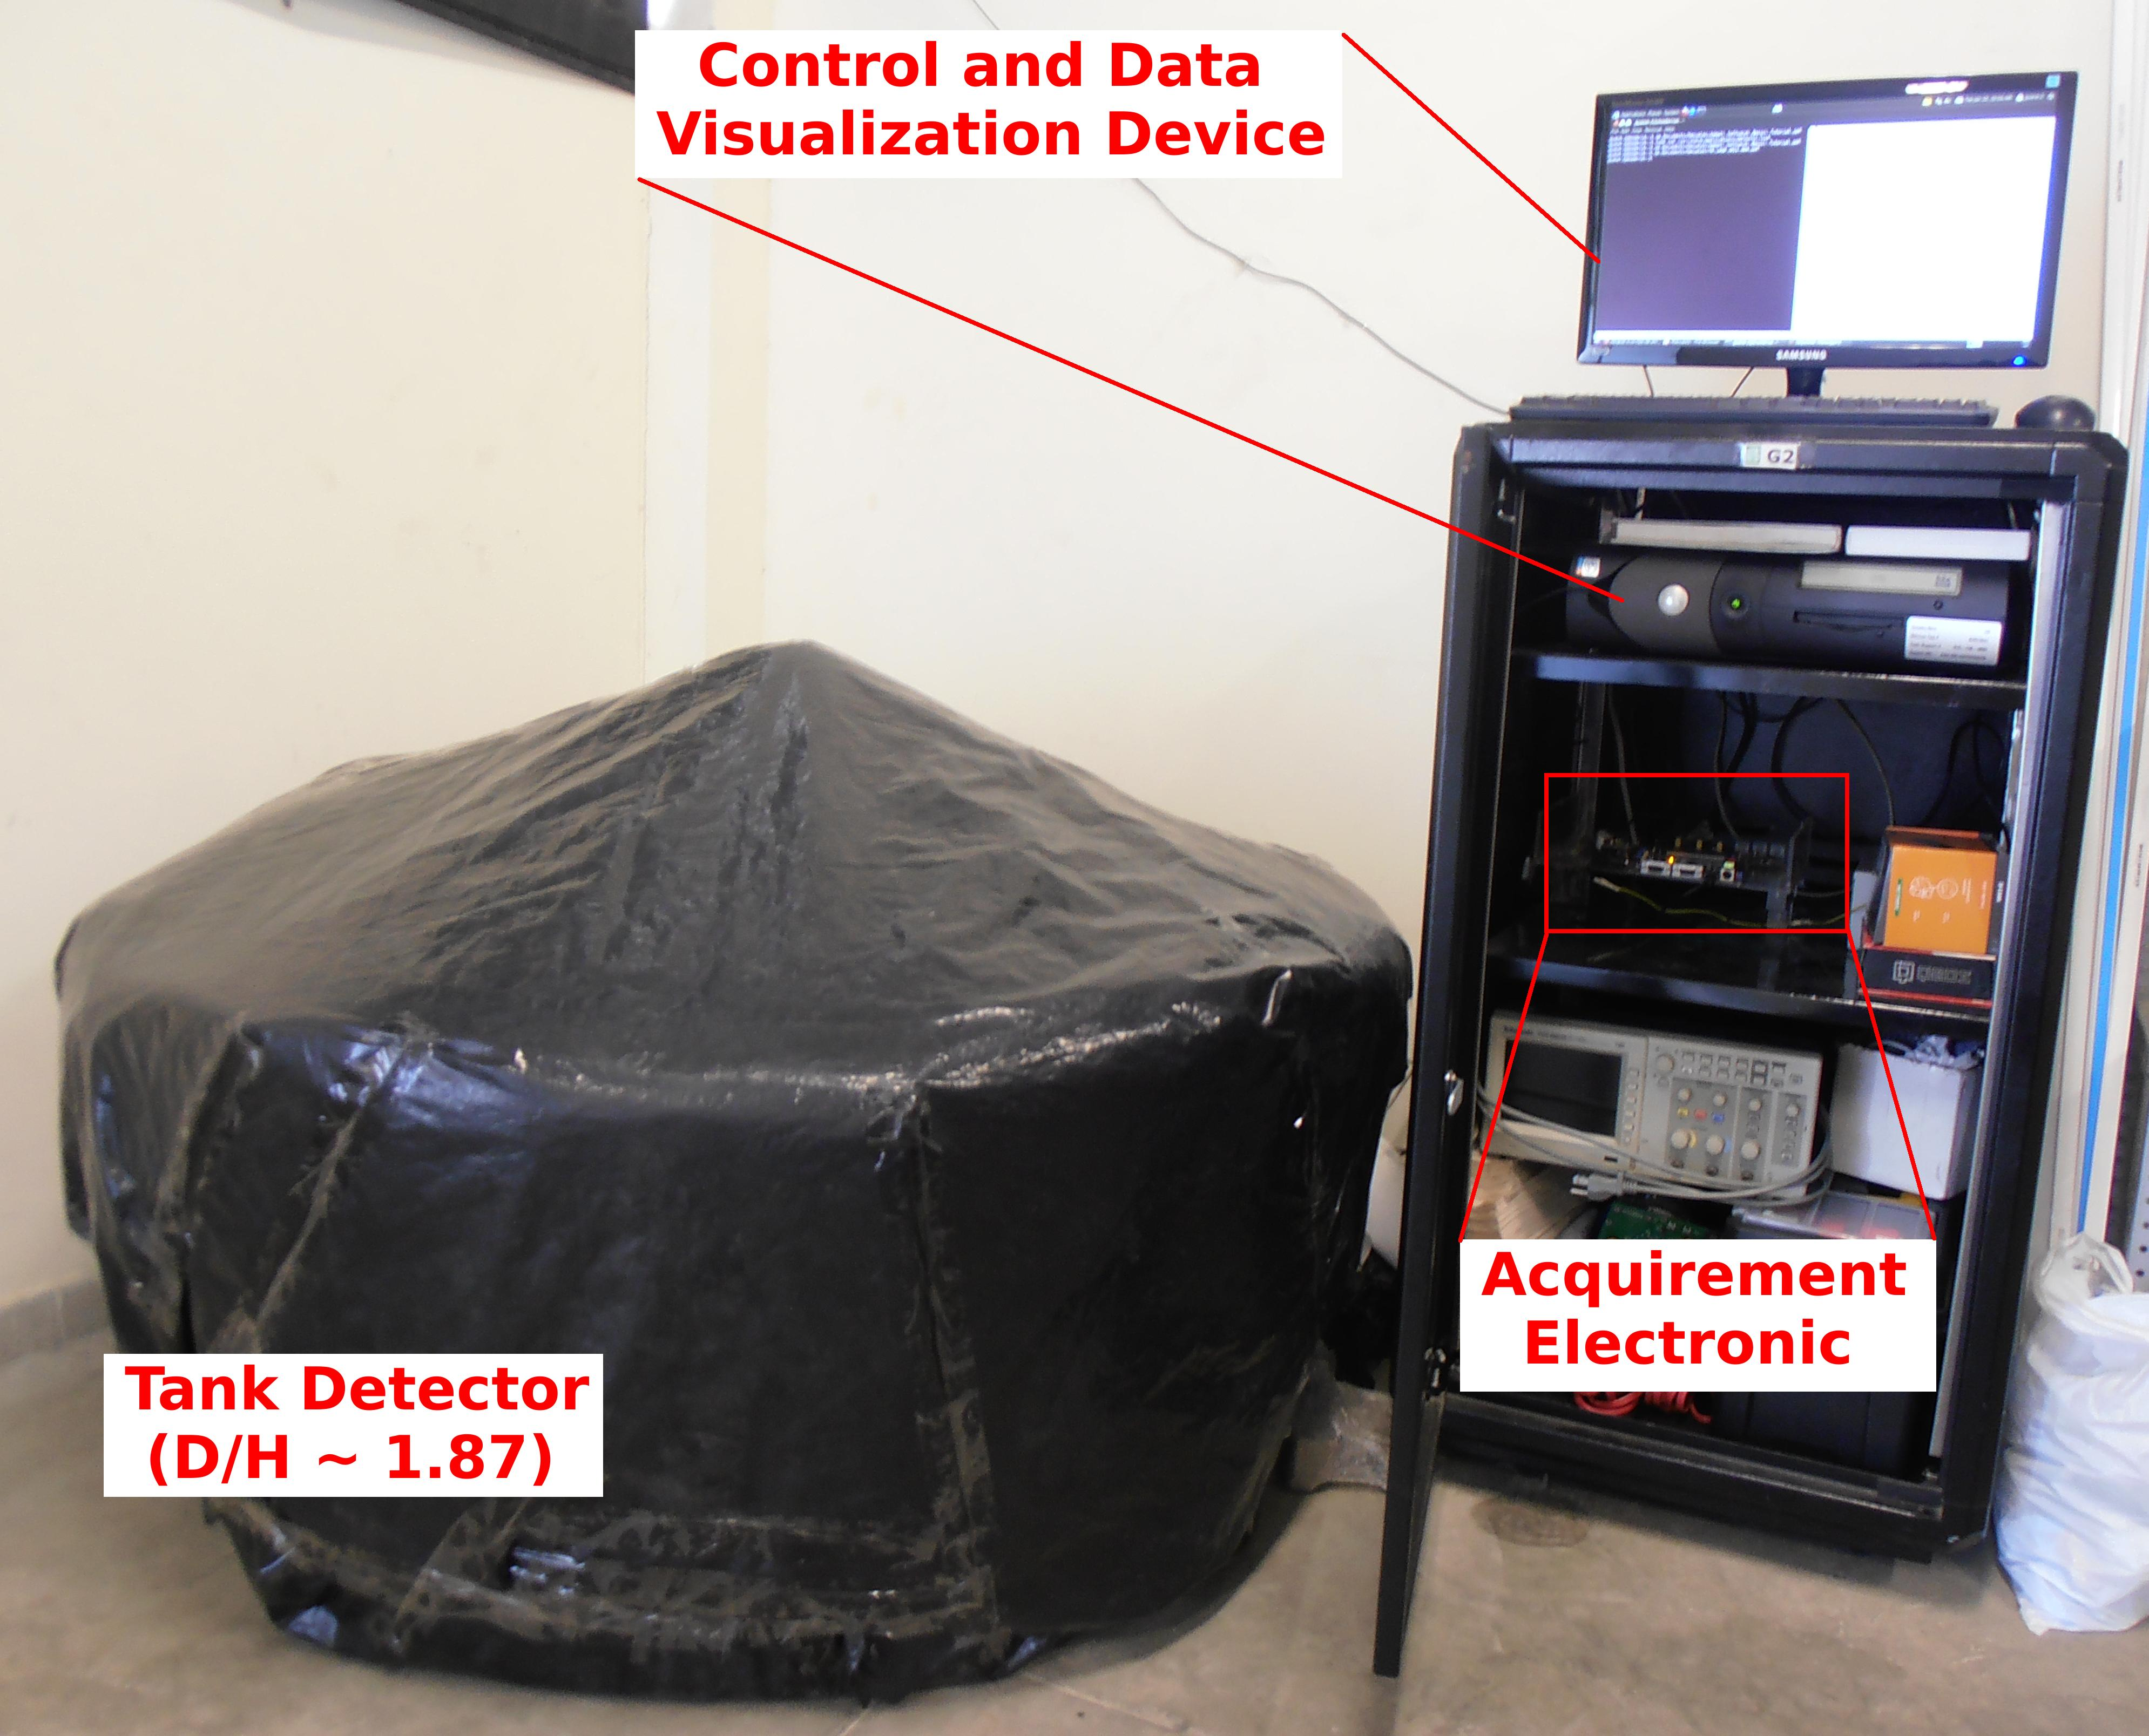
\includegraphics[width=3in]{figuresLAGOPaper2013/WCD-Guane3.jpg}
\caption{GUANE-3 WCD at Bucaramanga-Santander (7.140143 lat, -73.121904 long and 956masl) }
\label{Guane3WCD}
\end{center}
\end{figure}

As in other LAGO WCD, the signal is digitized and readout by prototype electronics from the
Engineering phase from the collaboration, with custom made programming both 
of the DAQ CPU and of the low level FPGA trigger. Two components can be 
clearly distinguished: a commercial Nexys2 FPGA 1200 gates board and the Local 
Station, LS i.e, the analog-digital converter board (see Fig 
\ref{LAGOElectronics2011}). The converted PMT signal is digitized by the LS and sent to the external computer by usb connection.  The system has attached three sensors, namely GPS,
pressure and temperature and has been programmed to stamp theses data every 
second. The thresholds are set depending on the PMTs characteristics (gain and 
noise).

Figure \ref{Histcharge} displays simulated and real registered charge histogram for the GUANE-3 WCD, where the green line represent  Muon Montecarlo Simulations entering in Guane3 with cenit angles from $0$ to $60$ degrees. The superposition of both graph clearly identify the Vertical Equivalent Muon (VEM)\footnote{defined as the energy
deposited in the tank by 1GeV Muon that crosses it vertically} 
which is used to calibrate the detector.

As it is clear form Fig  \ref{MeanPulse}, pulses registered by Guane-3 have a particular shape: 
rapid increase and declining exponentially  

\begin{figure}
\centering
\subfigure[]
{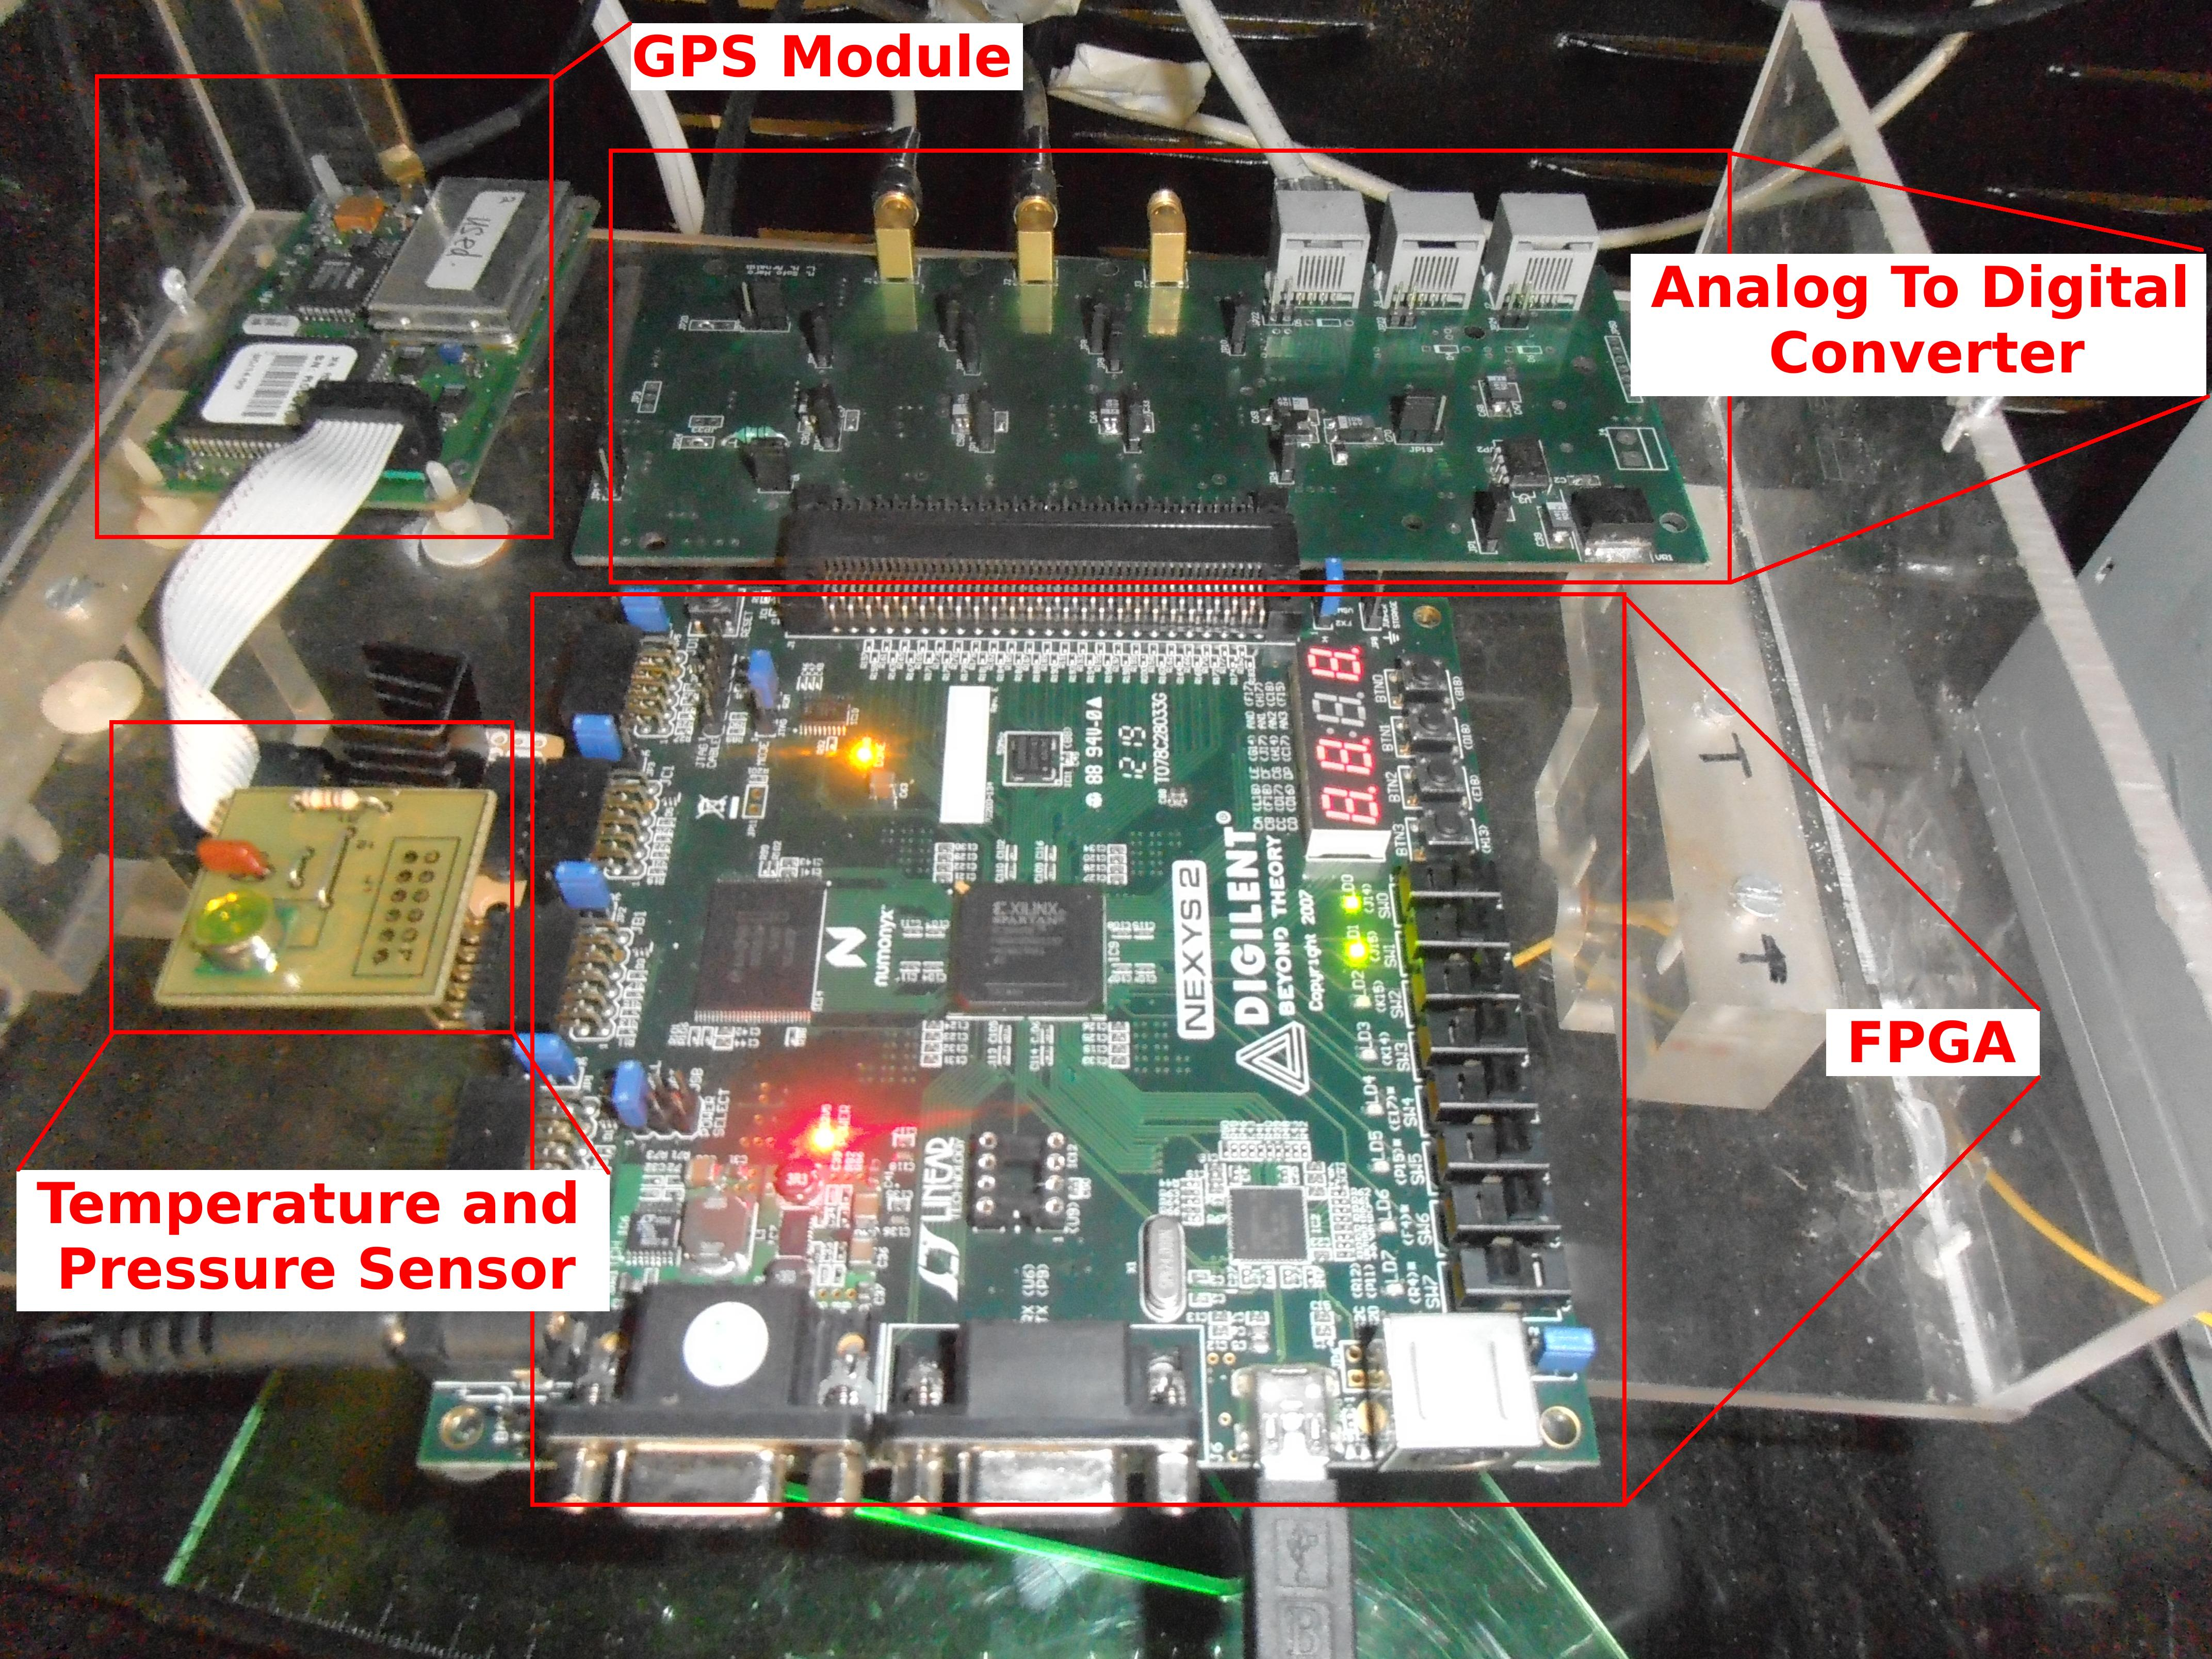
\includegraphics[width=3in]{figuresLAGOPaper2013/ElectronicDevice.jpg} \label{LAGOElectronics2011}}
\subfigure[]
{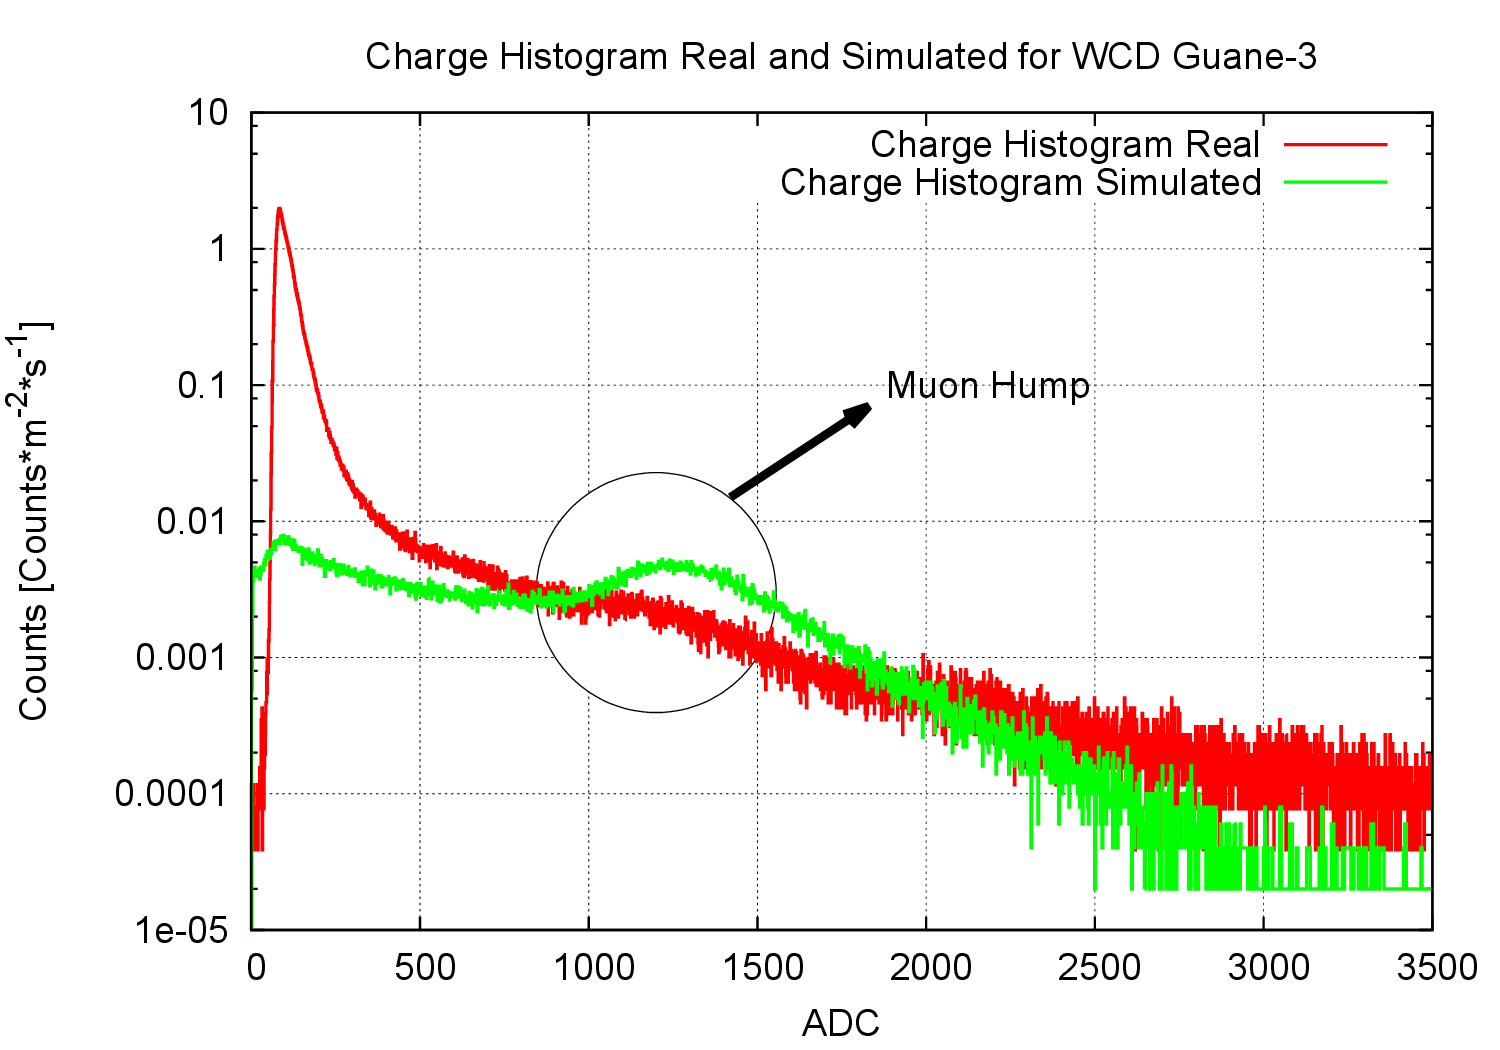
\includegraphics[width=3in]{figuresLAGOPaper2013/Histcharge-Guane3.png} \label{Histcharge}}
\subfigure[]
{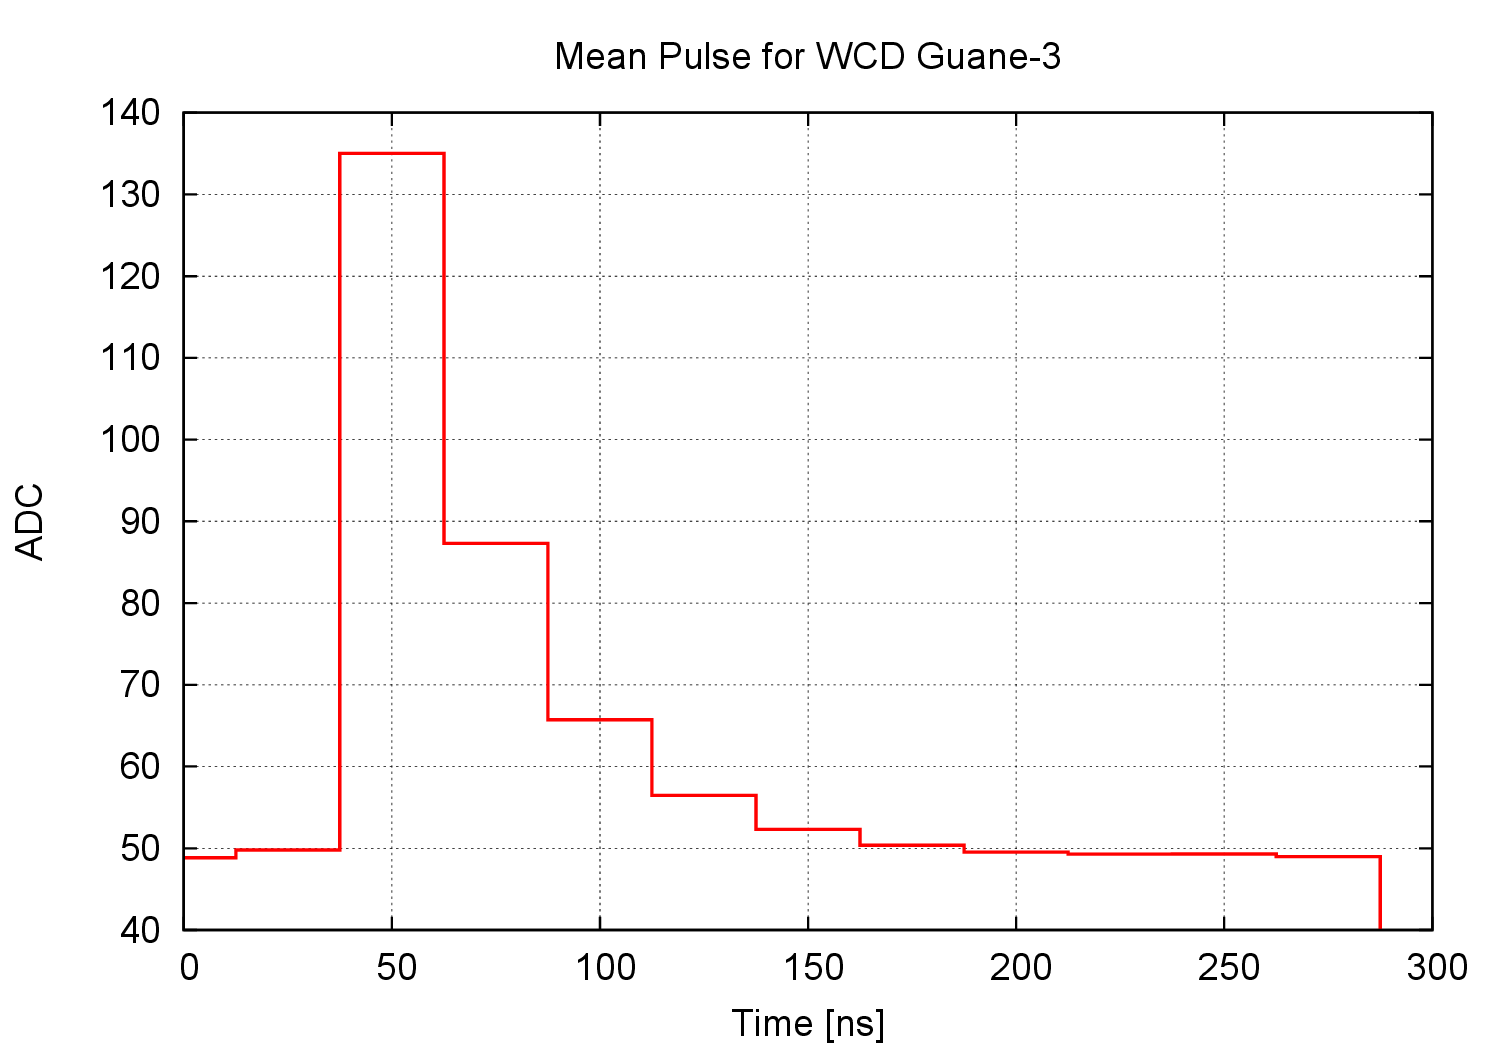
\includegraphics[width=3in]{figuresLAGOPaper2013/MeanPulse-Guane3.png} \label{MeanPulse}}
\caption{Plate \ref{LAGOElectronics2011} illustrates different parts of CAB-LAGO Electronics. Plate \ref{Histcharge} displays simulated and real charge histogram for the GUANE-3 WCD.  Finally, plate \ref{MeanPulse} } 
\end{figure}

\subsection{Calibration Curves}
Calibrating, operating and monitoring WCDs at high altitude and/or remote countryside places can be a significant complex task. The characteristic hump left by muons in a WCD (such as the one used for calibrating the Pierre 
Auger Observatory WCDs, see \cite{BertouEtal2006} is smeared by the large background of electrons, positrons and photons.
In order to calibrate Guane-3 WCD, it is standard to use the VEM \cite{EtchegoyenEtal2005}.
Thus this unit defines the high energy region ($>  1$ VEM) and the
low energy region ($ < 1$ VEM). The equivalence between VEM and ADC units,
can be obtained by comparing the charge histograms with the corresponding Montecarlo simulations. For our Guane-3 WCD we have $1$ VEM $\sim 1200$ ADC. 


\subsection{E-science and the data deluge}
Terms such as ``cyber-infrastructure'', ``e-science'' and, more
recently, ``e-research'' have been coined to describe this
knowledge revolution. Among its most distinctive features we
can cite: the intensive use of information and communication
technologies (ICT); geographically distributed resources for
information processing and analysis; and above all, its
ubiquitousness (see Refs. \cite{HeyTrefethen2003, Foster2005, HeyTrefethen2005} and
references therein). Its main challenge is to manage, analyze
and preserve the \textit{data deluge} caused by an impressive
variety of sensors, ambitious numerical simulations and
large-scale facilities such as particle accelerators, tokamaks,
synchrotron radiation sources and ground and satellite-borne
astronomical telescopes. Under this digital avalanche, which
surpasses any traditional data management capacity, ICT can
transform these instruments into powerful computer environments
for data mining.
A similar path is followed by small data producers scattered
around the globe; thus both large and small data producers face
the same problems in knowledge cataloging, preservation and
dissemination. It is imperative to plan and build repositories
that store data as they emerge and to retain the history of the
decisions and criteria that generate them \cite{GrayEtal2002, KarastiEtal2006,
BorgmanWallisEnyedy2007, Murray2008}.

Inspired by the reflections and conceptual
bases of the debutante, the Open Data Movement, LAGO Colombia has been developing two main initiatives to deploy a network of curated data repositories, namely:
\begin{enumerate}
  \item to preserve, curate and share the data registered by the large aperture WCD array, now through a data repository (DR) and in the near future across a network of DR
  \item to generate a toolkit of scripts and algorithms to detect the proper operation of the detector. This toolkit will part of the next generation of firmware and will allows the system to reconfigure some of its parameter in order to minimize some of diagnosed malfunctioning.  
 \item to offer a computational infrastructure that allows the collaboration members to ubicously analyze the curated data efficiently
\end{enumerate}
These initiatives aim to pave the way to openly share the data recorded with any other domain disciplines.

The reasons for preserving data derive from the fact that
observations, knowledge and understanding are cumulative. A
{\em datum} can be considered a piece of information that can
be processed, interpreted, transmitted and preserved. Data
arise either from measurements (observational or experimental
data), simulated results (synthetic data computed with
mathematical models) or historical records (historical data).
Data may be considered raw if they are generated directly from
measurements and models, or derived if they undergo further
filtering and processing
Adequate documentation
regarding sampling, analytical procedures, anomalies, accuracy
and structure is key in its future correct interpretation.
Metadata can facilitate \cite{MichenerEtal1997}:
\begin{itemize}
  \item data identification and acquisition for a given
      subject, for a specific period of time or geographic
      location;
  \item automatic analysis and data modeling;
  \item the inclusion of semantic knowledge elements
      associated with the data.
\end{itemize}
The incorporation of metadata demands an investment of time and
effort by those who generate, preserve and share the data. It
is advisable to make allocation for metadata-model definition
and for the implementation learning curve, followed by
maintenance costs in the short, medium and long term. For the
implementation of a metadata system to be successful, there
must be institutional commitment, i.e. the acceptance of
technical field staff, researchers, students and computer and
laboratory technicians.

There are different metadata standards available,
namely Dublin Core, Darwin Core, Content Standard for Digital
Geospatial Metadata, ISO 19115 Geographic information metadata,
Ecological Metadata Language, etc. The reason for so many
standards is the diversity of domain fields: information
science, biology, geology, ecology and cartography, to name but
a few.

\subsubsection{Data preserved, curated and shared}
The LAGO Colombia has developed a prototype of  data repository, \texttt{LAGOData} \cite{TorresEtAl2011} as a part of a more ambitious project,  \texttt{LAGOVirtual}\cite{CamachoEtal2009}, oriented to develop a working environment to have access and to analyzed the data recorded in all LAGO Sites. In \texttt{LAGOData}  repository the data are classified  into three types: instrument calibration data, WCD data sets and simulated data sets. In a near future we want the members of the collaboration use this repository also to preserve papers, thesis, Labs Notes and reports related with the project. The idea will be to link all mentioned data sets to the documents produced from the  corresponding data analysis.  

Each data file is tagged by a metadata set specifically adapted to LAGO. The existence and implementation of a scientific metadata standard model will allow an uniform access to data for all the members of LAGO colaboration, the interoperability between scientific information systems and also will contribute to the data preservation and its usability in time. The metadata model we propose for \texttt{LAGOData} is an adaptation of the model raised for the Council for the Central Laboratory of the Research Councils \cite{Sufi2004}

We have developed a prototype of the data repository for the LAGO collaboration adapting the system  DSpace  \cite{SmithEtal2003}, an open source software that enables open sharing of many types of content, generally used for institutional repositories.  Dspace can expose the data and metadata through the Open Archives Initiatives Protocol for Metadata Harvesting\footnote{\url{http://www.openarchives.org/OAI/2.0/openarchivesprotocol.htm}} (\cite{VanSopelEtal2004}) . This protocol is used  by external systems to collect the data and metadata and create services of aggregated value like meta-searchers. Also offers the data through Really Simple Syndication channels, RSS, which is available at all levels in the structure of the repository. These channels are a simple mechanism to show the contents recently submitted. The detailed description of the implementation of this data repository based on DSpace can be found elsewhere \cite{TorresEtAl2011} and an interesting survey of a hundred of DR can be found in ref \cite{MarcialHemminger2010}.

We expect to release a second version of \texttt{LAGOData} for mid 2014 which will have an implementation of the SWORD ( for \textit{Simple Web-service Offering Repository Deposit}  ) protocol which became a way to address the need for a standardised deposit interface to digital repositories \cite{LewisDeCastroJones2012}. With this implementation  we will be not only able to synchronize a network of DR across all LAGO site, but also to automatically stamp a basic metada each data set collected at each WCD of the LAGO Collaboration.
 
\begin{figure}[h!]
\centering
\subfigure[]
{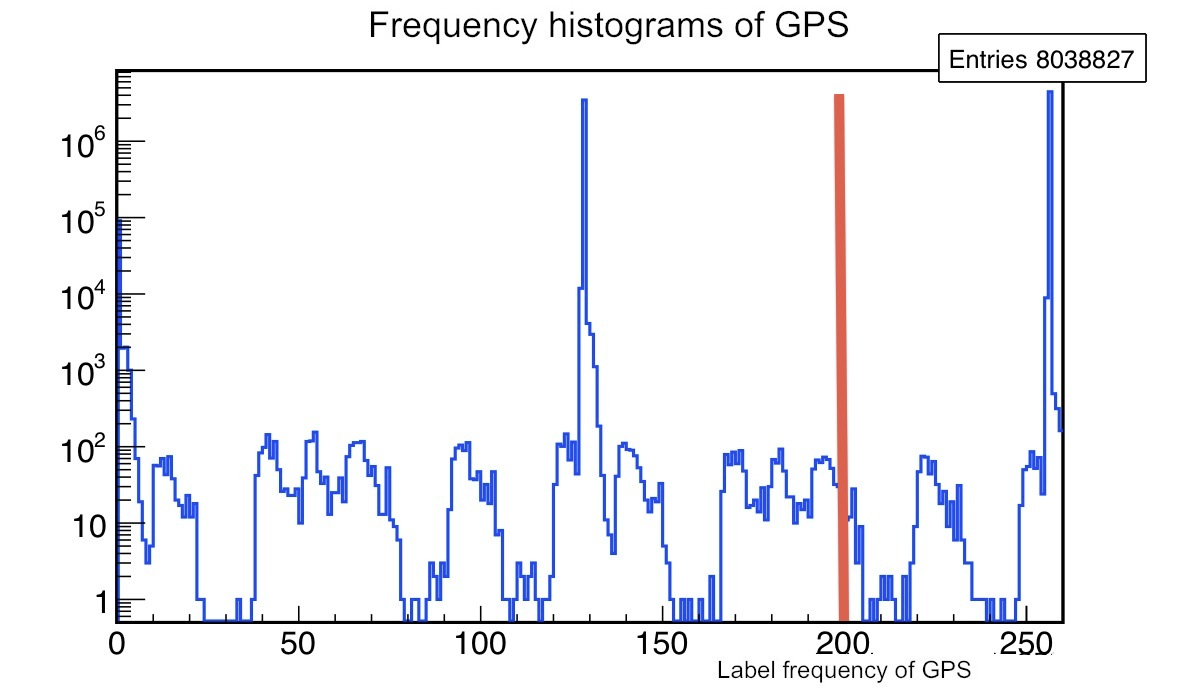
\includegraphics[width=3in]{figuresLAGOPaper2013/SN_Final_2008.jpg} \label{SN2008} }
\subfigure[] 
{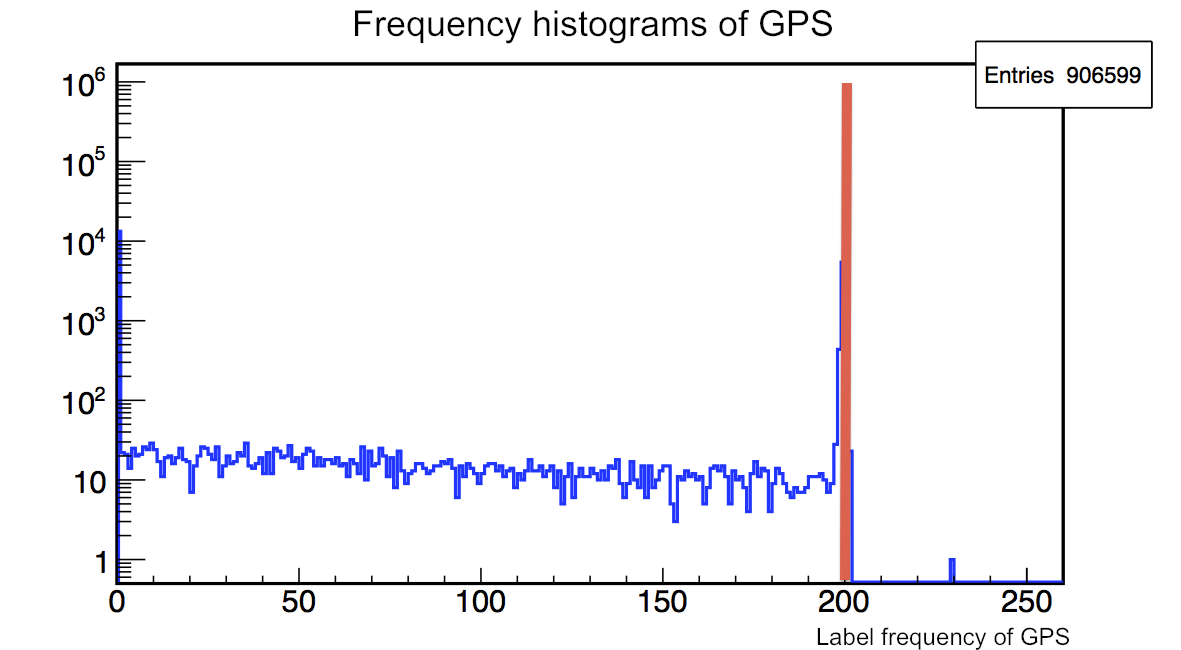
\includegraphics[width=3in]{figuresLAGOPaper2013/CHA_final_histo_2011.png} \label{CH2011}}

\caption{ This figure shows histograms for the GPS clock marks. Figure \ref{SN2008} represents the GPS clock marks recorded at one of the Sierra Negra, Mexico WCD, while  Fig \ref{CH2011} display the frequency of recording data for one WCD at Chacaltaya, Bolivia. The red column in these histograms represents the ideal GPS clock mark distribution. Horizontal arrows illustrate deviation from the ideal distribution.}
\label{dataQuality}
\end{figure}


\subsubsection{Data-Driven Instrumentation and Data quality}
The notion of data-driven instrumentation is an emerging new concept for the IT world, but absolutely  familiar for the astronomical communities where adaptive optical telescopes have been profited for almost a decade (see \cite{Roddier1999,Tyson2010} and references there in). These are reconfigurable instruments that can be self-adapted to new situations induced by external data inputs.  LAGO Colombia has been working generating a set of tools,  scripts and algorithms to give the detectors some intelligent resources of intelligence in order to enable them to diagnosis the appropriateness of their operation. This toolkit will part of the next generation of firmware of the WCD electronic and will allows the system to reconfigure some of its parameter in order to minimize some of diagnosed malfunctioning.   

In order to guarantee the quality of the data emerging from the WCD we have developed several simple scripts to check the correctness of the operation of the detecting electronics. These tools contrast the ideal pattern time series with the real data arrangement coming from the detector.  

The ideal data file should have 200 GPS clock marks per second, i.e. the electronics records the signals from the PMT. 200 times per second.  This is the ideal way to record data and it is represented in figures  \ref{SN2008} and  \ref{CH2011} with a red column. Figure \ref{SN2008} represents the GPS clock marks recorded, during the year 2008, at one WCD from LAGO site at Sierra Negra, Mexico. It is clear how different is from the ideal recording (red column) because most commons clock marks at 128 and 256, but not at 200. On the other hand, Fig \ref{CH2011} displays the frequency of recording data for one WCD at Chacaltaya, Bolivia. In this case the electronics records signals from the PMT closer to the ideal operating frequency (see a more detailed analysis in \cite{NunezQuinonezSarmiento2013}).

 Additionally, LAGO the electronics is very sensible to atmospheric electromagnetic disturbances. Typically thunderstorms, that generate severe change in pressure, temperature  and other weather electric disturbances which can be associated with antipulses or high variations in voltage. These ghost signals produced by intense variation on the recording whether variables (or environmental electric fields) have to be excluded  from curated data sets. To identify and remove ghost signals on the curated data sets we have performed an sliding time window analysis looking for signals having 3$\sigma$ deviations from the average. The sliding window analysis, is an standard strategy where statistical parameters are calculated for a small frame, or window, of the data. The window incrementally advances across the surveyed region and, at each new position, an the new statistical indicators are calculated. In our case, we have selected $60s$ as a frame window, with a sliding increment of $0.2s$. The analysis was performed over all data files, from Sierra Negra and Chacaltaya LAGO sites, that passed the above criterium of the 200 GPS clock marks. We had found and remove two ghost signals produced by a significant variations of the electronics baseline. Those data sets that comply with both above criteria (200 clock marks and no ghost signals) are called Good Run List and are available at the LAGO DR \cite{Sarmiento2012}.
 
 \begin{figure}
\begin{center}
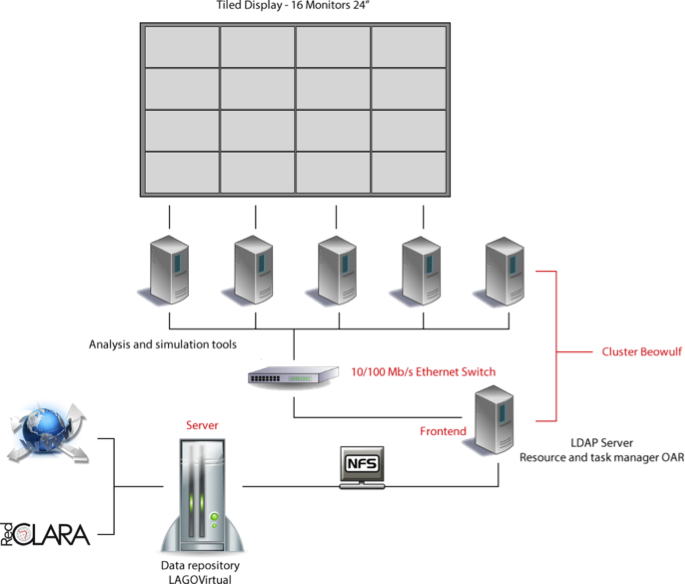
\includegraphics[width=3in]{figuresLAGOPaper2013/ComputationalLAGOInfra.png} 
\caption{First level of LAGOColombia Computational infrastructure}
\label{LAGOCompInfra}
\end{center}
\end{figure}

\subsubsection{LAGO Computational Infrastructure}
LAGO Colombia has been working to provide advanced computational support for the rest of the collaboration. This is a two level of computational (hardware \& software) infrastructure is represented, firstly by a local small dedicated cluster with an advanced visualization interface and secondly some tools available at the supercomputer center of the Universidad Industrial de Santander. The small dedicated cluster is a six Workstation (Quad Core Intel Xeon E5520, 4 GB RAM/node and 2 TB DD/node) with NVIDIA Quadro NVS 420 which controls a visualization wall of 16 monitors of 24 inches, capable to generate a resolution of 32 MP (see Fig \ref{LAGOCompInfra}).  

The Collaboration has been granted with an access to supercomputer facilities from the Universidad Industrial de Santander. Several applications are there available for the collaboration.

\textcolor{red}{Hern'an, cuales aplicaciones tenemos disponibles en cada sitio}

\section*{Acknowledgements}
LAGO Colombia gratefully acknowledge for the financial support of the Vicerrector\'ia de Investigaci\'on y Extensi\'on de la Universidad Industrial de Santander. The LAGO Collaboration has been benefited from the advanced computational infrastructure provided by the Centro de Supercomputaci\'on y C\'alculo Cient\'ifico (SC3) de la Universidad Industrial de Santander. We are also in debt of the financial support of RedCLARA funding support through the ALICE2 project and form the International Centre for Theoretical Physics under the External Office Activities programs. 

\begin{thebibliography}{10}

\bibitem{Suarez2011}
M.~Suarez.
\newblock Instalaci\'on de un detector cherenkov de agua para la detecci\'on de
  trazas de rayos c\'osmicos a 956 metros sobre el nivel del mar.
\newblock Master's thesis, Escuela de F\'isica, Universidad Industrial de
  Santander, Colombia, 2011.

\bibitem{BertouEtal2006}
X.~Bertou, P.S. Allison, C.~Bonifazi, P.~Bauleo, C.M. Grunfeld, M.~Aglietta,
  F.~Arneodo, D.~Barnhill, J.J. Beatty, N.G. Busca, A.~Creusot, D.~Dornic,
  A.~Etchegoyen, A.~Filevitch, P.L. Ghia, I.~Lhenry-Yvon, M.C. Medina,
  E.~Moreno, D.~Nitz, T.~Ohnuki, S.~Ranchon, H.~Salazar, T.~Suomijarvi,
  D.~Supanitsky, A.~Tripathi, M.~Urban, and L.~Villasenor.
\newblock Calibration of the surface array of the pierre auger observatory.
\newblock {\em Nuclear Instruments and Methods in Physics Research Section A:
  Accelerators, Spectrometers, Detectors and Associated Equipment}, 568(2):839
  -- 846, 2006.

\bibitem{EtchegoyenEtal2005}
A.~Etchegoyen, P.~Bauleo, X.~Bertou, C.B. Bonifazi, A.~Filevich, M.C. Medina,
  D.G. Melo, A.C. Rovero, A.D. Supanitsky, and A.~Tamashiro.
\newblock Muon-track studies in a water cherenkov detector.
\newblock {\em Nuclear Instruments and Methods in Physics Research Section A:
  Accelerators, Spectrometers, Detectors and Associated Equipment}, 545(3):602
  -- 612, 2005.

\bibitem{HeyTrefethen2003}
T.~Hey and A.~E. Trefethen.
\newblock e-science and its implications.
\newblock {\em Phil. Trans. R. Soc. Lond. A}, 361:1809--1825, 2003.

\bibitem{Foster2005}
I.~Foster.
\newblock Service-oriented science.
\newblock {\em Science}, 308:814--817, May 2005.

\bibitem{HeyTrefethen2005}
T~Hey and A.~E. Trefethen.
\newblock Cyberinfrastructure for e-science.
\newblock {\em Science}, 308:817--821, May 2005.

\bibitem{GrayEtal2002}
J~Gray, A~Szalay, A~Thakar, and C~Stoughton.
\newblock Online scientific data curation, publication, and archiving.
\newblock In {\em SPIE Astronomy Telescopes and Instruments}, pages 103+107,
  Hawaii, 2002. Waikoloa.

\bibitem{KarastiEtal2006}
H.~Karasti, K.~Baker, and E.~Halkola.
\newblock Enriching the notion of data curation in e-science: Data managing and
  information infrastructuring in the long term ecological research (lter)
  network.
\newblock {\em Computer Supported Cooperative Work (CSCW)}, 15(4):321--358,
  August 2006.

\bibitem{BorgmanWallisEnyedy2007}
C~Borgman, J~Wallis, and N~Enyedy.
\newblock Little science confronts the data deluge: habitat ecology, embedded
  sensor networks and digital libraries.
\newblock {\em Int J Digit Libr}, 7:17--30, Jan 2007.

\bibitem{Murray2008}
P~Murray-Rust.
\newblock Open data in science.
\newblock {\em precedings.nature.com}, 2008.

\bibitem{MichenerEtal1997}
W~Michener, J~Brunt, J~Helly, T~Kirchner, and SG~Stafford.
\newblock Nongeospatial metadata for the ecological sciences.
\newblock {\em Ecological Applications}, 7(1):330--342, Jan 1997.

\bibitem{TorresEtAl2011}
L.A. Torres, L.A. Nu{\~n}ez, R.~Torr{\'e}ns, and E.H. Barrios.
\newblock Implementaci�n de un repositorio de datos cient\'{\i}ficos usando
  dspace.
\newblock {\em E-Colabora}, 1(2):101--117, 2011.

\bibitem{CamachoEtal2009}
R.~Camacho, R.~Chac{\'o}n, G.~D{\'\i}az, C.~Guada, V.~Hamar, H.~Hoeger,
  A.~Melfo, L.~A. N{\'u}{\~n}ez, Y.~P{\'e}rez, C.~Quintero, M.~Rosales, and
  R.~Torr{\'e}ns.
\newblock Lagovirtual. a collaborative environment for the large aperture grb
  observatory.
\newblock In R.~Mayo, H.~Hoeger, L.~Ciuffo, R.~Barbera, I.~Dutra, P.~Gavillet,
  and B.~Marechal, editors, {\em Proceedings of the Second EELA2 Conferencem
  Choron{\'\i} Venezuela}, Madrid Espa{\~n}a, 2009. EELA2, CIEMAT.

\bibitem{Sufi2004}
Shoaib Sufi and Brian Mathews.
\newblock Cclrc scientific metadata model: Version 2.
\newblock {\em Final report. Council for the Central Laboratory of the Research
  Councils. Report No: DL-TR-2004-001}, 2004.

\bibitem{SmithEtal2003}
MacKenzie Smith, Mary Barton, Mick Bass, Margret Branschofsky, Greg McClellan,
  Dave Stuve, Robert Tansley, and Julie~Harford Walker.
\newblock Dspace: An open source dynamic digital repository.
\newblock 2003.

\bibitem{VanSopelEtal2004}
Herbert Van~de Sompel, Michael~L Nelson, Carl Lagoze, and Simeon Warner.
\newblock Resource harvesting within the oai-pmh framework.
\newblock {\em D-lib magazine}, 10(12):1082--9873, 2004.

\bibitem{MarcialHemminger2010}
Laura~Haak Marcial and Bradley~M Hemminger.
\newblock Scientific data repositories on the web: An initial survey.
\newblock {\em Journal of the American Society for Information Science and
  Technology}, 61(10):2029--2048, 2010.

\bibitem{LewisDeCastroJones2012}
Stuart Lewis, Pablo de~Castro, and Richard Jones.
\newblock {SWORD: Facilitating Deposit Scenarios}.
\newblock {\em D-Lib Magazine}, 18(1-2), January 2012.

\bibitem{Roddier1999}
Fran{\c{c}}ois Roddier.
\newblock {\em Adaptive Optics in Astronomy}.
\newblock Cambridge university press, 1999.

\bibitem{Tyson2010}
Robert Tyson.
\newblock {\em Principles of Adaptive Optics}.
\newblock CRC Press, 2010.

\bibitem{NunezQuinonezSarmiento2013}
LA~N\'u\~nez, F.~Qui\~nonez, and C.~Sarmiento.
\newblock Validaci�n del linaje de los datos de la colaboraci�n lago.
  instalaciones sierra negra y chacaltaya.
\newblock {\em ITECKNE}, 10(1):104--112, 2013.

\bibitem{Sarmiento2012}
C.~Sarmiento.
\newblock Identificaci\'on de destellos gamma en los repositorios de datos de
  la colaboraci\'on lago.
\newblock Master's thesis, Escuela de F\'isica, Universidad Industrial de
  Santander, Bucaramanga - Colombia, 2012.

\end{thebibliography}


\end{document}  


In a sliding window analysis, these statistics are calculated for a small frame, or window, of the data. The window incrementally advances across the surveyed region and, at each new position, the reported statistics are calculated for the polymorphism data contained within the window. In this way, variation of each statistic across the surveyed region can be measured. This type of analysis allows one to investigate how patterns of variation change across a surveyed genomic segment; it is typically applied to the detection of local signatures of natural selection or the identification of local changes in mutation or recombination rates (e.g., hot spots of mutation or recombination).
